\documentclass[12pt]{report}
% pre\'ambulo

\usepackage{lmodern}
\usepackage[T1]{fontenc}
\usepackage[spanish,activeacute]{babel}
\usepackage{mathtools}
\usepackage[utf8]{inputenc}
\usepackage{cite}
\usepackage{graphicx}
\usepackage{float}
\usepackage{enumerate}

\graphicspath{ {imagenes/} }

\title{\bfseries Software de Apoyo al Análisis Radiológico de Tomográfias Computarizadas}
\author{León Díaz Raúl Alberto\\ Osnaya Gómez Alexis Alan\\ Ríos López José Alberto\\ Santiago Nieves Edgar Augusto\\ \\}

\begin{document}

\maketitle 
\chapter{Introducción}

\section{Antecedentes}
En el año de 1972 se publicó en la revista \textit{British Journal of Radiology} un artículo del ingeniero Sir Godfrey Newboold Hounsfield sobre una técnica basada en rayos X, llamada tomografia computarizada, la cual hacía uso de métodos matemáticos desarrollados una decada antes por A. M. Cormack.
El nuevo método propuesto realizaba una división de la cabeza en varios cortes los cuales irradiaban a través de sus bordes, por lo cual la radiación emitida podía ser aislada dentro de la misma porción. La ventaja que este método presentaba frente a la técnica convecnional de rayos X, era que la información no presentaba alteraciones debidas al material presente a los lados del corte en cuestión.\\ \\
Con el fin de superar a la radiología convencional, el nuevo método pretendía superar 3 limitantes; la primera, la imposibilidad de mostrar toda la información de una escena tridimensional en una imagen radilógica bidimensional, debido a la superposición de los objetos en la imagen obtenida; la segunda limitante a vencer era la escaza capacidad de distinguir los tejidos blandos; finalmente, no era posible cuantificar las densidades que tenían los tejidos.\cite{TCFundamentos}  \\ \\
Con el surgimiento de la tomografía computarizada y otras modalidades de diagnóstico digital con imágenes  el ACR(American College of Radiology) y el NEMA(National Electrical Manufacturers Association) se dieron cuenta que se debía crear un método estandar para la transferencia de imagenes e información asociada a está, entre dispositivos de diferentes fabricantes. En 1993 surge DICOM(Digital Imaging and Communication in Medicine) como un estandar ante la problemática planteada.\cite{DICOMNEMA} \\

\section{Planteamiento del problema}
Hoy en día las tomografías computarizadas son herramientas muy útiles en el campo médico biológico sin embargo no siempre se aprovecha el potencial de toda la información que se puede obtener con este tipo de estudios pues las herramientas de edición en los visores utilizados en estos procedimientos hacen un análisis sobre la imagen y no sobre los datos por lo cual el ínidce de fiabilidad de los resultados disminuye. Las aplicaciones que hacen un buen uso de la información obtenida desde las tomografías computarizadas son poco accesibles debido a su alta complejidad además de sus elevados costos. Al omitir ésta información se pueden pasar por alto algunas particularidades de la imagen que van desde tumores en etapa temprana hasta metástasis. \\

\section{Propuesta de solución}
Para dar solución a la problemática anteriormente planteada se propone diseñar y desarrollar una herramienta de reconstrucción de estructuras internas del cuerpo humano y clasificación por densidades de los tejidos a partir de la matriz de datos obtenida a través tomografías axiales computarizadas contenidas en un archivo de tipo DICOM, la cual permitirá a médicos y radiólogos una fácil interpretación de  los resultados.

El primer paso será la decodificación de un archivo DICOM, el segundo realizar un conjunto de técnicas que permitan hacer un análisis de la imagen para posteriormente aplicar algoritmos de clasificación y agrupamiento, finalmente se presentará la información generada de manera gráfica.

En la figura 1.1 se observa el diagrama general de funcionamiento del sistema.
\begin{figure}[H]
\centering
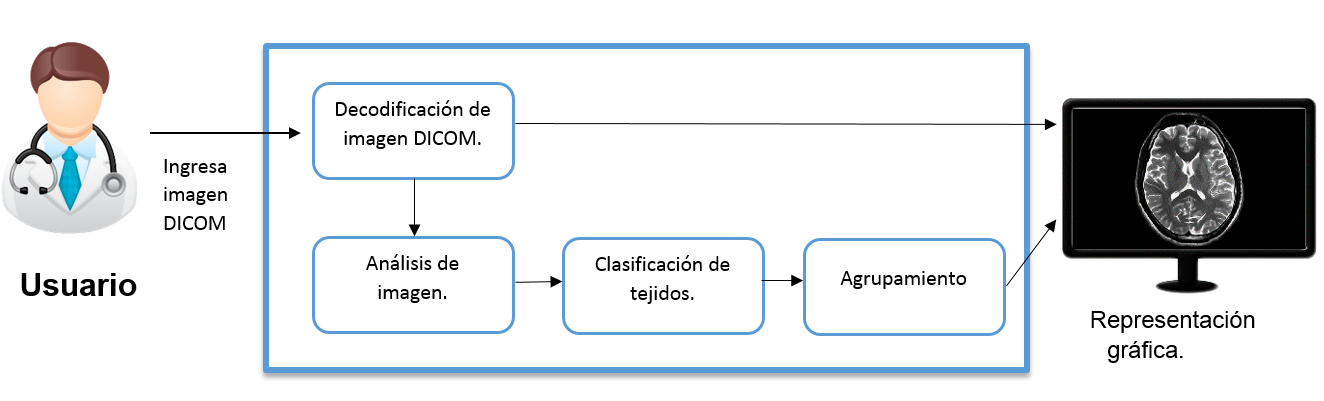
\includegraphics[width = 13 cm, height = 5 cm]{diagramageneral}
\caption{Diagrama del funcionamiento del sistema}
\end{figure}

\section{Justificación}
A lo largo de los años la evolución de la ciencia y la tecnología han permitido que el campo de la medicina se desarrolle y avance en un gran nivel, al permitir el desarrollo de medicinas y aparatos quirúrgicos que facilitan y minimizan el error dentro de los procesos, desafortunadamente no en todos los campos del área esto se ha logrado, cuando hablamos de errores médicos debemos tomar en cuenta que las consecuencias que estos pueden traer son muy delicadas pues en muchas ocasiones representan la vida o muerte de los pacientes.\\ \\
“La interpretación de los estudios tomográficos radiológicos se realiza comúnmente con base en un análisis visual de las imágenes adquiridas de los equipos imageneológicos por parte del médico radiólogo, estos análisis son susceptibles a malas interpretaciones debido a error humano”, por esto es que decidimos realizar este trabajo con el fin de ayudar a la interpretación de estos estudios.
Las técnicas de segmentación y umbralización aplicadas sobre los datos de una imagen DICOM permitirán un mejor análisis de las tomografías.\\ \\
Este TT beneficia a la sociedad en general pues cualquiera puede necesitar un estudio por medio de una TAC y gracias al software propuesto se visualizará la densidad de los tejidos para saber así el estado de estos.

\section{Objetivos}
\subsection{Onjetivo General}
Desarrollar un software que permita realizar un análisis y clasificación de tejidos con base en los resultados obtenidos a partir de tomografías axiales computarizadas en formato DICOM, para el apoyo en la interpretación de estudios radiológicos a la comunidad médica especializada.
\subsection{Objetivos Particulares}
\begin{itemize}
\item Leer e interpretar la información contenida en una imagen DICOM.
\item Clasificacr por densidades distintos tipos de tejidos presentes en las imágenes.
\item Reconstruir estructuras internas del cuerpo mediante aplicación de técnicas de análisis de imagen y algoritmos de clasificación y agrupamiento.
\item Facilitar la interpretación de tomografías mediante un visor.
\end{itemize}


\chapter{Marco teórico}
En este capítulo se detallarán algunos terminos que ayudarán a una mayor compresión del funcionamiento del sistema.
\section{Estado del arte}
La solución que se propone ante la problemática planteada no es una solución completamente nueva pues se han desarrollado anteriormente otros softwares que poseen una idea similar pero se atacan con un enfoque diferente. A continuación se listan algunos sistemas y trabajos similares a la propuesta realizada.

\hfill\break
\textbf{\textit{Image Analysis Software}}
\\Algunas características ofrecidas por el software son las siguientes:
\begin{itemize}
\item Analiza modelos celulares complejos.
\item Gestiona eficazmente grandes cantidades de datos.
\item Visualiza modelos de células en 2D o 3D en tiempo real.
\item Muestra tejidos y cuantfica celulas.
\end{itemize}

\hfill\break
\textbf{\textit{3D-Doctor}}
\\El software proporciona las siguiente características:
\begin{itemize}
\item Puede leer imagenes DICOM, TIFF, BMP, JPEG, Interfile, PNG, PGM, GIF.
\item Contiene modelos 3D de exportación STL(ASCII y binario), 3D Studio(3DS)entre otros para l rápida creación de prototipos.
\item Mide área, superficie 3D, volumen 3D, distancia, perfil y región de un histograma.
\item Representación de diferentes tejidos.
\item Imagenes 3D CT/MRI pueden ser cortadas de nuevo facilmente a lo largo de un eje arbitrario.
\item Corte de imágenes para corregir las rebanadas de grosor desigual, el redimensionado de volumen y la rotación de imagen.
\end{itemize}

\hfill\break
\textbf{\textit{Análisis digital de imágenes tomográficas sin contraste para la busqueda de tumores cerebrales}}
\\La tesis presentada nos ofrece estas características:
\begin{itemize}
\item Análisis digital de imágenes y reconocimiento de patrones para la busqueda de tumores cerebrales.
\item Codificación y ectracción de la imagen a partir del archivo digital proporcionada por los sistemas PACS de la actualidad.
\end{itemize}


\hfill\break
\textbf{\textit{Reconstrucción tridimensional de estructuras internas del cuerpo humano a partir de tomografías axiales computarizadas}}
\\Las características de este trabajo terminal desarrollado en la Escuela Superior de Cómputo se presentan a continuación:
\begin{itemize}
\item Sistema de reconstrucción tridimensional de estrucuturas internas del cuerpo humano mediante tomografías computarizadas(TAC) en formato DICOM(''Digital Imaging and Communication in Medicine''). Dicho sistema proporcionará una amplia manipulación del objeto generado en 3D.
\end{itemize}

\section{Imagen}
Una imagen es una colección de medidas en dos o tres dimensiones espaciales. En imagenes médicas estas medidas o ''intensidades'' pueden ser absorción de radiación  en imagenes de rayos X, presión acúsitca en ultrasonidos o ampllitud de señal de radiofrecuencias en resonancias magnéticas. Si cada posición de la imagen tiene una única medida, la imagen es llamada ''imagen escalar''. Si las posiciones tienen más de una medida se les llama ''imágenes vectoriales'' o ''multicanal''. Las imágenes pueden ser adquiridas en un dominio continuo, como en la películas de rayos X, o en un espacio discreto como en las resonancias magnéticas. En las imágenes discretas en 2D la localiazción de cada medida es llamada ''pixel'' y en imagenes 3D se llama ''voxel''. Por simplicidad usaremos el termino ''pixel'' para ambos tipos de imagen 2D y 3D.

\section{Imágenes médicas}
Una imagen médica es un conjunto de técnicas y procesos usados para crear imágenes del cuerpo humano, o partes de él, con propósitos clínicos  o para la ciencia médica.\\
Representa gráficamente una distribución espacial de una o más propiedades físicas o químicas del interior del cuerpo humano. Dos de los parámetros mayor importancia son el contraste y la resolución. \\
El contraste se define como la diferencia en la intensidad entre un punto de  la imagen y determina lo que podemos ver en la imagen, en el caso del contraste en una imagen medica es muy importante tener el conocimiento de diversos parámetros físicos o químicos que ayuden a entender lo que está siendo representado.\\
La resolución por su parte se define como la nitidez con la que se percibe una imagen observada por un instrumento óptico. Nos ayuda a encontrar todas las características de la imagen para así distinguir y analizar detalles.\cite{essen} \\ \\
Modalidades de las imágenes médicas.\\
\begin{itemize}
\item Radiología: Es el uso médico de la radiación para diagnosticar y tratar diversos problemas de salud. A partir de la utilización de rayos gamma, rayos X y otras clases de rayos, es posible obtener imágenes internas del organismo.
\item Medicina nuclear: Es una especialidad médica que realiza diagnósticos y tratamientos mediante la utilización de trazadores o radiofármacos. Realiza estudios de órganos y sistemas desde el punto de vista funcional.  La Medicina Nuclear se diferencia de las otras técnicas de imagen en que realiza estudios fisiopatológicos. Es decir da una visión de cómo funciona el organismo.
\item Ecografía: Utiliza ondas sonoras de alta frecuencia para observar órganos y estructuras al interior del cuerpo.
\item Resonancia magnética: Se considera como una técnica no invasiva, ya que no requiere la introducción de herramientas o elementos en el cuerpo ni tiene consecuencias para el paciente. La información que se obtiene a través de la resonancia magnética es convertida en imágenes en una computadora (ordenador), permitiendo que el profesional observe, de este modo, el interior del organismo.
\item Endoscopia: Es un procedimiento que permite que el médico vea el interior de su cuerpo. Utiliza un instrumento llamado endoscopio o tubo visor. Los endoscopios tienen una cámara diminuta unida a un tubo largo y delgado.
\end{itemize}

\section{Tomografía computarizada}
Es un procedimiento computarizado de imágenes por rayos X en el que se proyecta un haz angosto de rayos X a un paciente y se gira rápidamente alrededor del cuerpo, produciendo señales que son procesadas por la computadora de la máquina para generar imágenes transversales o cortes del cuerpo.\\
El descubrimiento y el desarrollo de la TC (Tomografía Computarizada) revolucionó el diagnóstico por imagen en medicina. La TC es una técnica digital y matemática de diagnóstico por imagen, que origina cortes tomográficos en los que cada capa no está contaminada por estructuras borrosas procedentes de la anatomía adyacente. Lo más importante, la TC permite la diferenciación y cuantificación de los tejidos duros y blandos. De este modo, por primera vez en las técnicas de imagen en medicina, el radiólogo podía visualizar los tejidos duros y blandos sobre una imagen, sin llevar a cabo un procedimiento invasivo sobre el paciente, como puede ser la inyección de medios de contraste.\\
La TC produce imágenes axiales de la anotomía de un paciente. Dichas imágenes se obtienen de forma perpendicular al eje mayor del cuerpo. La TC es una técnica de diagnóstico para imagen digital. La fuente de rayo X se une rígidamente a un dispositivo detector de la geometría en abanico de los rayos, que rota 360 grados alrededor del paciente y recoge los datos. El detector de imagen presenta un estado gaseoso o sólido, lo que produce señales que sirven como datos de entrada para un ordenador exclusivo. Dicho ordenador procesa los datos mediantes técnicas de retroproyección con algoritmo de Fourier, desarrolladas por primera vez por Hounsfield para dar lugar a imágenes de TC. Las imágenes de TC son en sí mismas tridimensionales, de 512 X 512 pixeles típicamente, con un espesor definido por la separación de cortes de la técnica de imagen. Cada elemento de la imagen de TC se denomina vóxel, el cual presenta un valor, al cual se le refiere en unidades de Hounsfield, que describe la densidad de la imagen de TC en dicho punto.\\
El resultado final de la reconstrucción por la computadora, es una matriz de números, que no es conveniente para su visualización en pantalla, por lo que un procesador se encarga de asignar a cada número o rango de números, un tono gris adecuado. Los valores numéricos de la imagen de tomografía computada, están relacionados con los coeficientes de atenuación, debido a que la disminución que sufre el haz de rayos X, al atravesar un objeto, depende de los coeficientes de atenuación lineales locales del objeto.\\
Algunas ventajas que ofrece esta técnica es el tiempo de exploración del orden de segundos en las modernas generaciones de aparatos, unido a su absoluto inocuidad (capacidad de hacer daño), lo que permite repetirlo cuantas veces sea necesario, así como si alta fiabilidad diagnóstica de certeza media, que alcanza el 85\%, superando con creces los resultados de todas las técnicas exploratorias
clásicas juntas, aunque, justo es decirlo, no las desplaza en absoluto, sino que todas ellas se complementas mutuamente.\\
Los posibles usos de este método diagnóstico, son los siguientes: anormalidades del cerebro y medula espinal, tumores cerebrales y accidentes cerebro vasculares, sinusitis, aneurisma de aorta, infecciones torácicas, enfermedades de órganos como el hígado, los riñones y los nódulos linfáticos del abdomen y muchos otros más.\\

\section{DICOM}
DICOM (Digital Imaging and Comunications in Medicine) es un estándar propuesto y administrado por la National Electrical Manufacturers Association (NEMA) en 1992. Especifica mecanismos de codificación, almacenamiento y transmisión de imágenes médicas; para llevar a cabo un análisis digital de imágenes médicas, generalmente se utilizan visores DICOM que implementan el estándar ya que con ellos es posible visualizar y exportar las imágenes a formatos de imagen digital comunes (JPG, PNG, BMP, etc.). 
El formato genérico del archivo de DICOM consiste en dos partes diferenciadas:
\begin{enumerate}
\item Una cabecera (header) con multitud de campos estandarizados que especifican datos administrativos (datos del paciente, hospital donde se realizó, entre otros), datos sobre el estudio y la sintaxis de transferencia UID  que específica la codificación y la compresión del conjunto de datos que le sigue.
\item Un conjunto de datos (data set) de DICOM, que contiene la imagen o las imágenes especificadas que pueden estar comprimidas con distintos estándares.
\end{enumerate}

\begin{figure}[H]
\centering
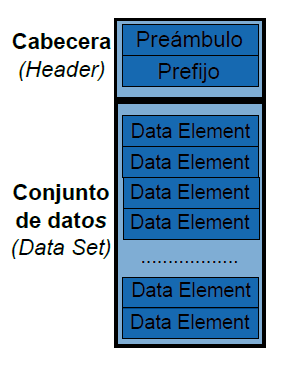
\includegraphics[width = 7 cm, height = 10 cm]{estructura}
\caption{Estructura de un archivo DICOM}
\end{figure}

Características del estándar DICOM
\begin{enumerate}
\item Puede aplicarse en una red mediante el protocolo de red TCP/IP.
\item Se puede almacenar en medios externos como CD-R y MOD y sistemas de archivo lógicos y
para PC.
\item Especifica la semántica de los comandos y los datos asociados mediante el concepto de Clases
de Servicios (Service Classes).
\item Incluye objetos de información para graficado de presiones por curvas, reportes, estudios,
pacientes, impresiones y otros grupos de datos.
\item Es posible identificar claramente cualquier Objeto de Información conforme son transmitidos
a través de la red.
\end{enumerate}




\section{Escala de Hounsfield}
El elemento individual de la imagen de TC es el vóxel, que tiene el valor, referido en unidades de Hounsfield, que describe la densidad de la imagen de TC en ese punto. Cada vóxel contiene 12 bits de datos y va desde -1000(aire) hasta los +3000 de unidades Hounsfield. Los escáneres de TC tienen un valor estandarizado de Hounsfield de 0 para el agua. La escala de densidad de los TC es cuantitativa y significativa en cuanto a la identificación y diferenciación de las estructurad y los tejidos.\\
La escala de Hounsfield (HU) es una transformación lineal de la medida original del coeficiente de atenuación, basada en la rediodensidad del agua destilada, establecido en el STP (estándar presión y temperatura) y se define como igual a 0HU, mientras que la radiodensidad del aire en STP se define como -1000HU; lo anterior proporciona al tejido óseo más denso (hueso compacto) valores cercanos a +1000HU. La figura 1 muestra los números de TC aproximados para algunos tejidos y órganos comúnmente estudiados.\\
La escala Hounsfield se extiende a lo largo de 2000 unidades que difícilmente es distinguible si se le asignara a cada unidad, un nivel de brillo distinto en una monitor de vídeo, esto debido a que el ojo humano no es capaz de distinguir más de 40 tonalidades de brillo diferentes, representar en una imagen toda la gama de valores de la escala de Hounsfield, conlleva a no poder visualizar una gran cantidad de información. Por lo tanto, solo se representa mediante una escala de grises un sector parcial de los valores de TC con el fin de solo visualizar el órgano o tejido estudiado y su detalle.\\
\begin{figure}[H]
\centering
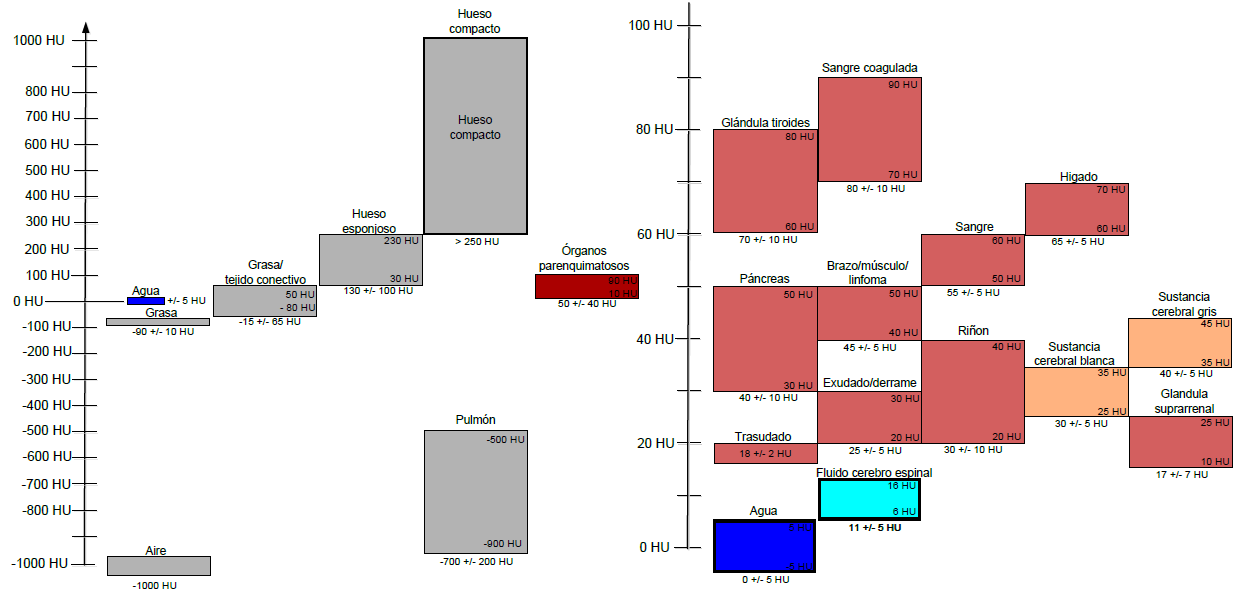
\includegraphics[width = 13 cm, height = 10 cm]{escala}
\caption{Escala de Hounsfield}
\end{figure}



\section{Segmentación}
La segementación de imágenes está definida como el particionado de una imagen en regiones constituyentes que no se solapan y las cuales son homogeneas con respecto a alguna característica como intensidad o textura. Si el dominio de la imagen está dado por $\Omega$, el problema de la segmentación es determinar cuales conjuntos $S_{k} \subset \Omega$, cuya unión, es el dominio $\Omega$ completo. Así, los conjuntos que componen una segmentación deben satisfacer \begin{equation} \Omega = \bigcup_{k = 1}^{K} S_{k} \end{equation}
donde $S_{k} \bigcap S_{j} = \o$ for $ k \neq j$ y cada $S_{k}$ está conectado. En un funcionamiento ideal, los métodos de segmentación encuentran aquellos conjuntos que corresponden a distintas estructuras anatómicas o regiones de interés en la imagen.\\
Si no tomamos en cuenta la restricción que indica que las regiones estén conectadas el proceso de determinar los conjuntos $S_{k}$ es llamado ''clasificación de pixeles'', y los conjuntos se llaman ''clases''. 
La clasificación de pixeles es una meta deseable en las imagenes médicas, especialmente cuando regiones desconectadas que pertenecen a la misma clase de tejido deben ser identificadas. Determinar el número total  de clases \textit{K} en la clasificación de pixeles puede ser un gran problema. 
A menudo, suponemos que el valor de \textit{K} se conoce con base en el conocimiento previo de la anatomía considerada. Por ejemplo, en la segmentación de una imagen cerebral obtenida a partir de una resonancia magnética, es común asumir que \textit{K} = 3, correspondiente a las clases de los tejidos de materia gris, materia blanca y el fluido cerebroespinal.\\
El etiquetado es el proceso de asignar un significado importante a cada región o clase, este procedimiento se puede llevar a cabo como un proceso separado de la segmentación. En este proceso se mapea el índice numérico \textit{k} del conjunto $S_{k}$ a una denominación anatómica. En la imagenología médica, las etiquetas por lo general son visualmente detectables con obviedad y pueden ser determinadas en una revisión por un físico o un técnico. El etiquetado automatizado por computadora son deeseables cuando las etiquetas no son obvias y en sistemas con procesos automatizados. Una típica situación que involucra etiquetado sucede en las mastografías digitales, en la cual la imagen es segmentada en diferentes regiones, las cuales después son clasificadas como sanas o tejido con tumor.

\subsection{Umbralización}
Las ténicas de umbralización segmentan imágenes escalares al generar una partición binaria a través de las intensidades de la imagen. La figura \textit{2.3a} muestra el histograma de una imagen escalar que aparentemente posee 3 clases, correspondientes a las 3 modas. El procedimiento de umbralización trata de determinar un valor de intensidad, llamado ''umbral'', el cual separa las clases deseadas. Logramos la segmentación cuando agrupamos los pixeles con intensidades mayores a las del umbral en una clase y todos los otros en otra clase. Dos umbrales potenciales se observan en la figura \textit{3a} en el valle del histograma. Determinar más de un valor umbral es un proceso llamado multiumbralización.\\

\begin{figure}[H]
\centering
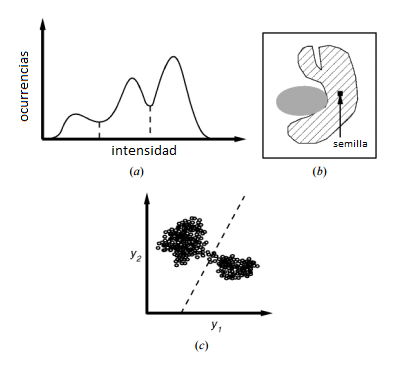
\includegraphics[width = 10 cm, height = 10 cm]{umbral}
\caption{Métodos de características espaciales y región creciente. (a)Histograma con 3 aparentes clases. (b)Característica espacial en 2-D. (c)Ejemplo de región creciente.}
\end{figure}

La umbralización es un procedimiento simple pero efectivo para segementar imagenes en las cuales diferentes estructuras tienen intensidades contrastantes u otras características cuantificables. A menudo la partición de la imagen se genera en interacción con el usuario aunque también existen métodos automatizados. A menudo, la umbralización se lleva a cabo interactivamente, basado en la asistencia visual del operador a partir la partición resultante.

La umbralización a menudo es utilizada como la primera de las operaciones en una secuencia de procesamiento de imagenes. Se ha aplicado en mastografías digitales, en las cuales usualmente hay presentes dos clases de tejidos --sanos y con tumores. Su principal limitación, es que en su forma más simple, sólo se generan dos clases y no se puede aplcar a imágenes multicanales. Además, la umbralización comunmente no toma en cuenta las características espaciales de la imagen. Esto causa que sea sensible a las inhomogeneidades de ruido e intensidad, lo cual puede pasar en la resonancia magnética. Ambos sucesos corrompen de manera significante el histograma de la imagen haciendo más difícil la separación. Por estas razones, se han propuesto variaciones a la umbralización clásica aplicada en imágenes médicas basadas en intensidades y conectividad. 

\subsubsection{Técnicas de umbralización.}
\textbf{ Técnicas Punto dependientes.}
\begin{enumerate}[A.]
\item \textit{Método de porcentaje.} En este método se asume que la imagen consiste de objetos oscuros en un fondo claro. Asumiendo que el porcentaje del objeto en el área es conocido, el umbral se define  como el nivel más alto de gris que mapea al menos $(100 - p)\%$ de los pixeles de los objetos de la imagen umbralizada. Este método no se puede aplicar a imagenes en las cuales no se conocen las áreas de los objetos.

\item \textit{Método modal.} Se utiliza en imágenes con distintos objetos y fondo, donde el histograma será bimodal. En este caso el umbral  se puede elegir como el nivel de gris existente en el valle del histograma. No se puede aplicar a imágenes con picos extremadamente diferentes o aquellas con valles anchos y planos.

\item \textit{Método Ostu.} Se basa en un análisis por discriminantes. En este método, la operación de umbral se considera como el particionado de los pixeles de la imagen en 2 clases $C_{0}$ y $C_{1}$ con base a un nivel de gris \textit{t}. Donde $C_{0} = \{0,1, ...,t\}$ y $C_{1} = \{t + 1, t +2, ..., l - 1\}$.


\item \textit{Método de análisis con base a la concavidad del histograma.} Cuando es posible encontrar el umbral mediante el valle del histograma es conveniente usar el método modal. En algunas imagenes aunque no sea posible hallar el valle, se puede obtener un buen umbral con base en las crestas del histograma. En aquellos casos donde ninguno de los anteriores es viables se toma en cuenta la concavidad del histograma, la cual está formada por la conjunción de los anteriores.

\item \textit{Métodos entrópicos.} En estos métodos recintemente desarrollados. el histograma de niveles de grises se considera como una fuente simbólica \textit{l}. El umbral óptimo se obtiene aplicando información de teoría. Algunoa ejemplos de estps métodos son los métodos de Pun, los métodos de Kapur, Sahoo y Wong, los de Johannsen y Bille, etc.

\item \textit{Método de preservación de momentos.} El valor del umbral es computado  determinísticamente de forma tal que los momentos de la imagen umbralizada queden en la imagen de salida(imagen binaria).

\item \textit{Método del error mínimo.} El histograma de nivel de grises  se ve como un estimado de la función de densidad de probabilidad $p(g)$ de la mezcla de población comprendida por los niveles de gris de los pixeles del objeto y del fondo.
\end{enumerate}

\textbf{ Técnicas Región dependientes.} 
\begin{enumerate}[A.]
\item \textit{Métodos de transformación de histogramas.} No se genera un umbral directamente si no que se transforma el histograma de nivel de grises a uno con crestas y valles más notorios en el cual se pueda aplicar alguno de los métodos de las técnicas punto dependientes.

\item \textit{Método de porcentaje.} A comparación de los métodos punto dependientes aquí se utilizan niveles de gris de segundo orden. Algunos  y ejemplos son la matriz de concurrencias y el método gráfico de dispersión(nivel de gris y nivel de gris local promedio).

\item \textit{Método de Deravi y Pal.} Se utilizan matrices de transición para definir dos ''medidas de interacción''. Se obtiene el umbral óptimo cuando se minimizan los valores de estas medidas.

\item \textit{Método de relajación.} Los pixeles se clasifican probabilisticamente en clases ''claras'' y ''oscuras'' basado en sus niveles de grises. Luego la probabilidad de cada pixel es ajustada con base en la probabilidad de los vecinos. El proceso se repite continuamente haciendo así mayor la probabilidad de que los pixeles claros pertenezcan a esa clase. 

\item \textit{Método de relajación de gradiente.} En el método de relajación de gradiente, el esquema de etiquetado óptimo se logra maximizando  los criterios de la función mediante optimización con gradiente.
\end{enumerate}

\textbf{ Umbralizado local.}\\
En el umbralizado local, la imagen origina se divide en imágenes más pequeñas y el umbral se determina para cada una de las imágenes obtenidas.

\textbf{ Métodos de multiumbralización.}
\begin{enumerate}[A.]
\item \textit{Método de segmentación de amplitud.} Utiliza las propiedades intrínsecas de la función de distribución acumulativa de una imagen para umbralizarla. La curvatura de la función de distribución es estudiada par obtener información relacionada a los valores de umbral.

\item \textit{Método de Wang y Haralick.} Primeramente los pixeles son clasificados como pixeles fronterizos o no fronterizos. Después, con base a sus vecinos se clasifican como relativamente claros u oscuros. Se obtiene un histograma de niveles de gris para aquellos pixeles fronterizos y relativamente claros y uno para los pixeles fronterizos relativamente oscuros. Se obtiene un valor de umbral basado en el nivel de intensidad de gris correspondiente a uno de los picos más altos de los dos histogramas.

\item \textit{Método de constraste uniforme.} Se crea un histograma del contraste promedio $\mu(t)$ para cada posible umbral $t$ y el pico más alto en el histograma es el umbral óptimo.
\end{enumerate}


\bibliographystyle{plain}
\bibliography{bibliografia}
\end{document}
